% \documentclass[aspectratio=169,notes]{beamer}
\documentclass[aspectratio=169]{beamer}
\usetheme[faculty=phil]{fibeamer}
\usepackage{polyglossia}
\setmainlanguage{english} %% main locale instead of `english`, you
%% can typeset the presentation in either Czech or Slovak,
%% respectively.
\setotherlanguages{russian} %% The additional keys allow
%%
%%   \begin{otherlanguage}{czech}   ... \end{otherlanguage}
%%   \begin{otherlanguage}{slovak}  ... \end{otherlanguage}
%%
%% These macros specify information about the presentation
\title[Artificial Intelligence Software (AIS)]{Artificial Intelligence Software, Lecture 4} %% that will be typeset on the
\subtitle{Model Selection and Sources
\\ \ \\ \  } %% title page.
\author{Oleg Bulichev}
%% These additional packages are used within the document:
\usepackage{ragged2e}  % `\justifying` text
\usepackage{booktabs}  % Tables
\usepackage{tabularx}
\usepackage{tikz}      % Diagrams
\usetikzlibrary{calc, shapes, backgrounds}
\usetikzlibrary{decorations.pathreplacing,calligraphy,calc,graphs}
\usepackage{amsmath, amssymb}
\usepackage{url}       % `\url`s
\usepackage{listings}  % Code listings
\usepackage{subfigure}
% \usepackage{floatrow}
% \usepackage{subcaption}
\usepackage{mathtools}
\usepackage{todonotes}
\usepackage{fontspec}
\usepackage{multicol}
\usepackage{pdfpages}
\usepackage{wrapfig}
\usepackage{qrcode}
\usepackage{animate}
\usepackage{booktabs}
\usepackage{multirow}
\usepackage{graphicx}
\usepackage{colortbl}

\graphicspath{{resources/}}
\frenchspacing

\setbeamertemplate{caption}{\raggedright\insertcaption\par}
\usetikzlibrary{graphs}

% \usepackage[backend=biber,style=ieee,autocite=footnote]{biblatex}
% \addbibresource{biblio.bib}
% \DefineBibliographyStrings{english}{%
%   bibliography = {References},}

\newcommand{\oleg}[2][] {\todo[color=red, #1] {OLEG:\\ #2}}
\newcommand{\fbckg}[1]{\usebackgroundtemplate{\includegraphics[width=\paperwidth]{#1}}}%frame background

\usepackage[framemethod=TikZ]{mdframed}
\newcommand{\dbox}[1]{
\begin{mdframed}[roundcorner=3pt, backgroundcolor=yellow, linewidth=0]
\vspace{1mm}
{#1}
\vspace{1mm}
\end{mdframed}
}

\begin{document}
\setlength{\abovedisplayskip}{0pt}
\setlength{\belowdisplayskip}{0pt}
\setlength{\abovedisplayshortskip}{0pt}
\setlength{\belowdisplayshortskip}{0pt}

\fbckg{fibeamer/figs/title_page.png}
\frame[c]{\setcounter{framenumber}{0}
    \usebeamerfont{title}%
    \usebeamercolor[fg]{title}%
    \begin{minipage}[b][6.5\baselineskip][b]{\textwidth}%
        \textcolor{black}{\raggedright\inserttitle}
    \end{minipage}
    % \vskip-1.5\baselineskip

    \usebeamerfont{subtitle}%
    \usebeamercolor[fg]{framesubtitle}%
    \begin{minipage}[b][3\baselineskip][b]{\textwidth}
        \raggedright%
        \insertsubtitle%
    \end{minipage}
    \vskip.25\baselineskip
}
%   \frame[c]{\maketitle}

\fbckg{fibeamer/figs/common.png}

\note{\scriptsize \begin{itemize}
        \item \
    \end{itemize}}


\begin{frame}[t]{Goal of the Lecture}
Given a task: <<\textbf{Find a model for Task X and run it}>>

\begin{center}
    \Large
    Our goal is to understand what a model is, what type of tasks exists, how to find it, what's important in it and how to launch it.
\end{center}
\end{frame}

\begin{frame}[t]{Architecture vs Weights}
\textbf{Architecture}
\begin{itemize}
\item Defines the computation graph (layers, connections)
\item Example: CNN, Transformer, MLP
\item Same architecture can be reused across tasks
\end{itemize}

\vspace{0.5em}

\textbf{Weights}
\begin{itemize}
\item Learned numerical parameters
\item Stored after training
\item Define the actual behavior of the model
\end{itemize}

\vspace{0.5em}

\textbf{Key idea:}
Same architecture + different weights = different models
\end{frame}

\begin{frame}[t]{What Does 2M / 85M Parameters Mean?}
    \begin{columns}[T,onlytextwidth]
        \begin{column}{0.49\textwidth}
            It's the number of learnable parameters.

\textbf{Interpretation:}
\begin{itemize}
\item 2M parameters $\rightarrow$ small model
\item 85M parameters $\rightarrow$ larger capacity
\item More parameters $\rightarrow$ more expressive, slower, heavier
\end{itemize}
        \end{column}
        \begin{column}{0.49\textwidth}
            \begin{figure}[H]
                \centering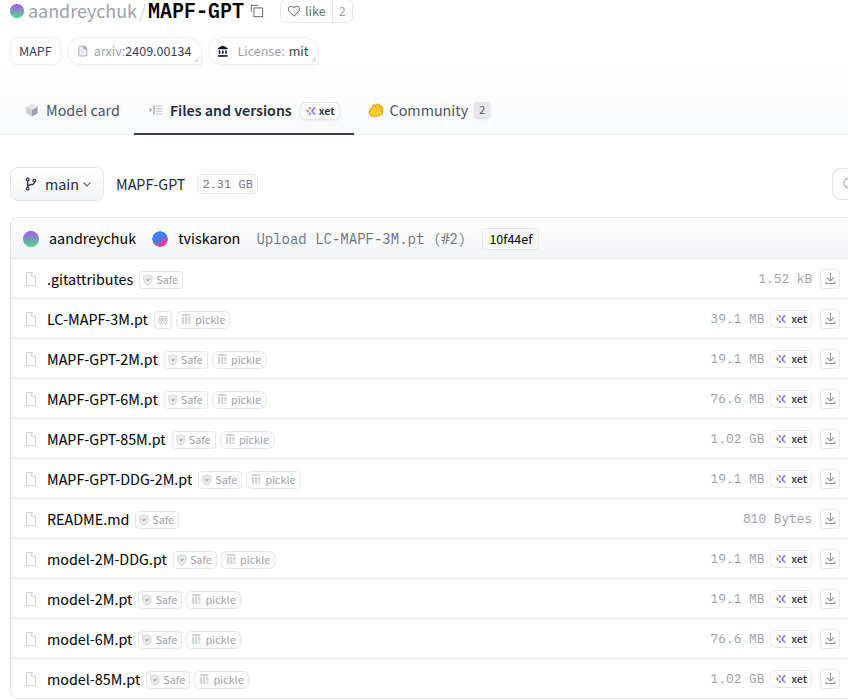
\includegraphics[height=5cm,width=1\textwidth,keepaspectratio]{diff_weights.png}
                % \caption{caption_name}
                \label{fig:diff_weights.png}
            \end{figure}
        \end{column}
    \end{columns}

\end{frame}

\begin{frame}[t]{How Can Models Share One Architecture?}
\begin{itemize}
\item Architecture defines the structure (e.g. ResNet18)
\item Parameters define the content inside this structure
\end{itemize}

\vspace{0.5em}

\textbf{Same architecture:}
\begin{itemize}
\item ResNet18 (ImageNet)
\item ResNet18 (medical images)
\end{itemize}

\vspace{0.5em}

\textbf{Differences:}
\begin{itemize}
\item Different weights
\item Different datasets
\item Different performance
\end{itemize}
\end{frame}

\begin{frame}[t]{Why Parameter Count Changes}
    \vspace*{-0.4cm}
\begin{itemize}
\item Depth (number of layers)
\item Width (number of neurons / channels)
\item Embedding size (Transformers)
\end{itemize}

\vspace{0.5em}

\textbf{Example:}
\begin{itemize}
\item ResNet18 vs ResNet50
\item YOLOv8n vs YOLOv8m vs YOLOv8l
\end{itemize}

\vspace{0.5em}

\textbf{Effect:}
\begin{itemize}
\item More parameters $\rightarrow$ better accuracy (usually)
\item More memory and compute
\item Slower inference
\end{itemize}
\end{frame}

\begin{frame}[t]{Unified Interface Across Models}
\begin{itemize}
\item Despite differences, models share a common pattern:
\end{itemize}

\begin{center}
\texttt{output = model(input)}
\end{center}


\textbf{Examples:}
\begin{itemize}
\item Image $\rightarrow$  classification scores
\item Text $\rightarrow$  sentiment label
\item Table $\rightarrow$  prediction
\end{itemize}

\vspace{0.5em}

\textbf{Important:}
\begin{itemize}
\item Interface is the same
\item Input format is NOT the same
\end{itemize}
\end{frame}

\begin{frame}[t]{Key Takeaways}
\begin{itemize}
\item Architecture = structure of computation
\item Parameters = learned knowledge
\item 2M / 85M = number of parameters
\end{itemize}

\vspace{0.5em}

\textbf{Main insight:}
\begin{itemize}
\item Same architecture can produce many models
\item Difference is in weights and scale
\end{itemize}

\vspace{0.5em}

\textbf{Practical view:}
\begin{itemize}
\item Models look similar in code
\item Real complexity is in data and preprocessing
\end{itemize}
\end{frame}

\begin{frame}[t]{Types of Tasks}
    \begin{columns}[T,onlytextwidth]
        \begin{column}{0.49\textwidth}
            \begin{itemize}
\item Computer Vision:
\begin{itemize}
\item classification
\item detection
\item segmentation
\end{itemize}
\item NLP (LLMs, embeddings)
\item Tabular (classification/regression)
\item Unsupervised (clustering)
\end{itemize}
        \end{column}
        \begin{column}{0.49\textwidth}
            \begin{figure}[H]
                \centering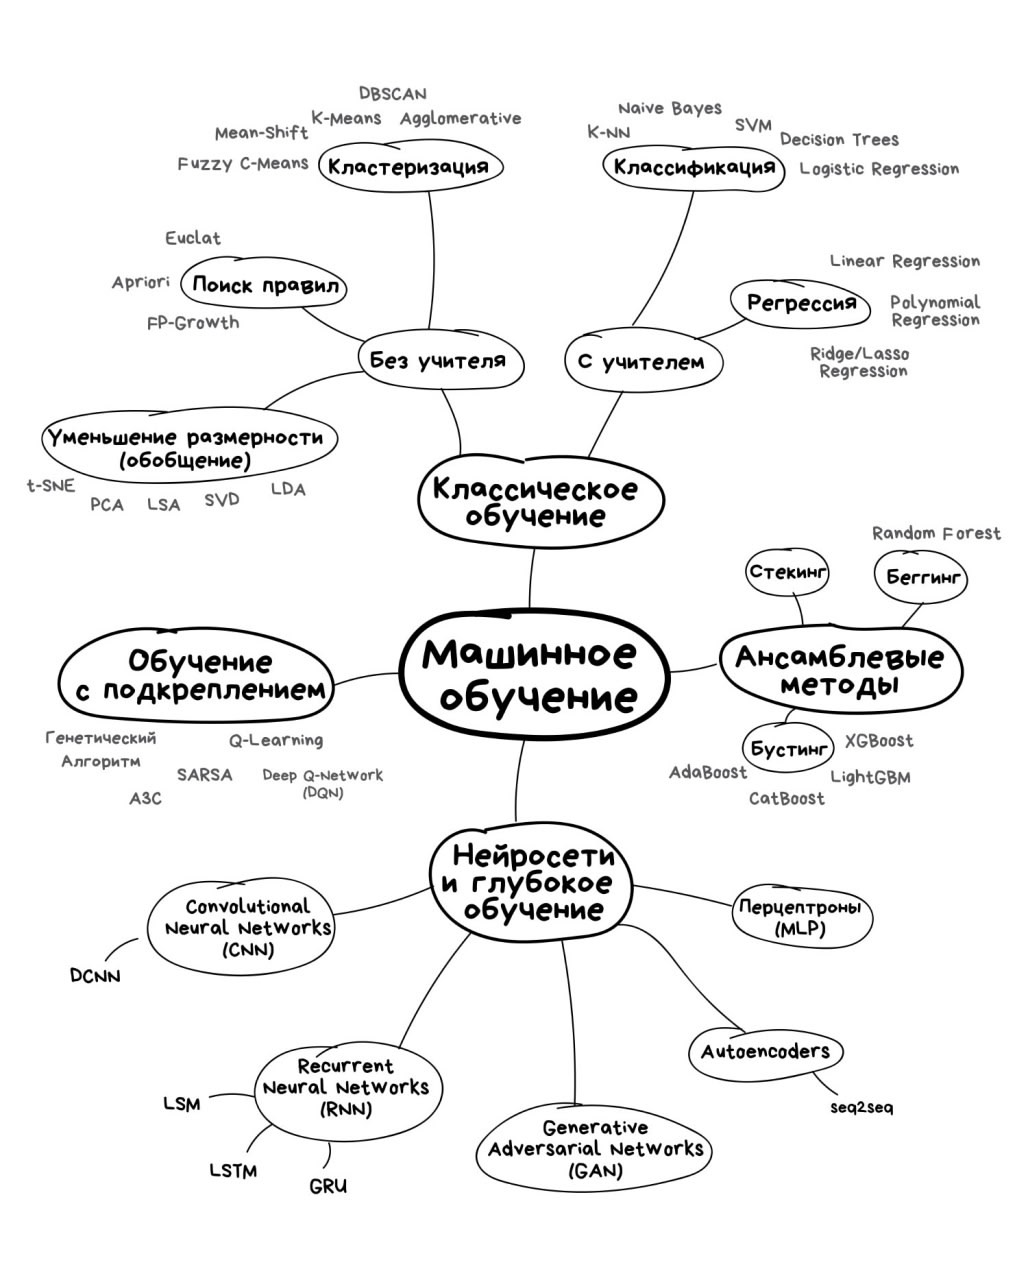
\includegraphics[height=5cm,width=1\textwidth,keepaspectratio]{task_types.png}
                % \caption{caption_name}
                \label{fig:task_types.png}
            \end{figure}
        \end{column}
    \end{columns}

\end{frame}

\begin{frame}[t]{Where to Find Models}
\begin{itemize}
\item \href{https://huggingface.co/models}{Hugging Face} — model hub for NLP, CV, multimodal
\item \href{https://github.com}{GitHub} — code and model implementations
\item \href{https://www.kaggle.com}{Kaggle} — notebooks and pretrained solutions
\item \href{https://pytorch.org/hub/}{Torch Hub} — PyTorch pretrained models
\item \href{https://arxiv.org}{arXiv} — research papers (often include models)
\item \href{https://ultralytics.com/}{Ultralytics YOLO} — ready-to-use CV models for detection and segmentation
\item \href{https://clear.ml/docs/latest/docs/model\_registry/}{ClearML Model Registry} — examples and versioned models for MLOps
\end{itemize}
\end{frame}

\begin{frame}[t]{Cloud Environments for Running Models}
\begin{itemize}
\item \href{https://huggingface.co/spaces}{Hugging Face Spaces} — deploy and run NLP, CV, and multimodal models in the cloud without local setup
\item \href{https://colab.research.google.com}{Google Colab} — free cloud notebooks with CPU/GPU, ready to run Python, PyTorch, TensorFlow
\item \href{https://www.kaggle.com/kernels}{Kaggle Kernels} — notebooks with preloaded datasets and pretrained models
\item \href{https://ultralytics.com/yolov8}{Ultralytics YOLO HUB} — online demos and inference for detection/segmentation
\item \href{https://clear.ml/docs/latest/docs/guides/clearml-task/clearml_task_tutorial/}{ClearML Tasks} — run training, inference, and manage models remotely with MLOps tools
\end{itemize}
\end{frame}

\begin{frame}[t]{Model = Code + Weights + Docs}
\begin{itemize}
\item Code: how to run
\item Weights: learned parameters
\item Docs: input/output format
\end{itemize}
\end{frame}



\begin{frame}[t]{How to Choose a Model}
\begin{itemize}
\item Input format
\item Output format
\item Metrics
\item Hardware requirements
\item Latency / size
\end{itemize}
\end{frame}



\begin{frame}[t]{Preprocessing Matters}
\begin{itemize}
\item Resize
\item Normalize
\item Tokenize
\item Channel order (RGB/BGR)
\end{itemize}

\textbf{Most errors come from wrong input}
\end{frame}

\begin{frame}{Examples}
\framesubtitle{}
    \Large all material in extra\_materials folder
\end{frame}

\begin{frame}[t]{Example: YOLO Detection}
\begin{itemize}
\item Input: image
\item Output: bounding boxes + labels
\item Postprocess: threshold, NMS
\end{itemize}
\end{frame}



\begin{frame}[t]{Example: NLP Pipeline}
\begin{itemize}
\item Input: text
\item Output: label + score
\item Tokenization inside pipeline
\end{itemize}
\end{frame}



\begin{frame}[t]{Classical ML Still Matters}
\begin{itemize}
\item Logistic Regression
\item Trees / Boosting
\item Fast and simple baselines
\end{itemize}
\end{frame}

\begin{frame}[t]{MLOps: Model Management with ClearML}
\begin{itemize}
\item \href{https://clear.ml/docs/latest/docs/model\_registry/}{Store models} — upload trained models to ClearML Model Registry for central access
\item \href{https://clear.ml/docs/latest/docs/webapp/webapp_model_viewing/}{Model Details} — ready-to-use example projects showing model storage, retrieval, and deployment
\end{itemize}
\end{frame}


\fbckg{fibeamer/figs/last_page.png}
\frame[plain]{}

\end{document}
